\chapter{Results}

In this chapter, the results are exposed in the following way: Section \ref{dset_section} shows how the dataset has been created and the overall proportion of classes. Section \ref{mono} is reserved to comparison and evaluation of monolithic machine learning models, Decision Tree, K-Nearest Neighbors, Multi Layer Perceptron, Naive Bayes and Support Vector Machine. For Multiple Classifier System (MCS), the Section \ref{mcs} compares the KNORAE, KNORAU, META-DES, OLA, Single Best and Static Selection. After the comparison between Monolithic and MCS, the overall comparison is discussed in Section \ref{result_ending}.

Using the dataset described in Section \ref{dset_section} other 30 different datasets have been randomly sampled that are subdivided into two: 80\% of the original dataset for model training and 20\% to test the model effectiveness. This method intends to make a Hypothesis Test, this help to statically evaluate if a classifier is really effective when applied in this dataset. After the classifiers applied to each of the 30 datasets, the mean and standard deviation of each metric are calculated and displayed in the result tables. For each classification method, both Monolithic and MCS have its setup described in Sections \ref{mono} and \ref{mcs} to ease future replications of this work. 

Each classifier is evaluated with 4 different metrics, precision (equation \ref{precision}), recall (equation \ref{recall}), F1 score (equation \ref{f1}) and accuracy (equation \ref{accuracy}). The precision is the ratio of correctly predictions to the total predictions done. Accuracy is the ratio of correctly true predictions to the total of predictions. Recall is the ratio of correctly positive predictions to all the predictions of a class. F1 score represents the harmonic mean between precision and recall, which is a more meaningful metric than the mean between precision and recall \cite{sasaki2007truth}. True positives are all instances of a class $C$ that are correctly classified. True negatives are all instances that do not belong to $C$ and are correctly classified. False positives of a class $C$ are the instances of other classes that has been classified as $C$. False negatives are instances of $C$ that has been classified as not belonging to $C$.

\begin{multicols}{2}%
    \noindent%
    {%
    \begin{equation} \label{precision} precision = \frac{TP}{TP+FP} \end{equation}%
    \begin{equation} \label{recall} recall = \frac{TP}{TP+FN} \end{equation}%
    }%
    {%
    \begin{equation} \label{f1} F1 = \frac{2 \times recall \times precision}{recall + precision} \end{equation}%
    \begin{equation} \label{accuracy} accuracy = \frac{TP+TN}{TP+TN+FP+FN} \end{equation}%
    }%
\end{multicols}

\section{Dataset}\label{dset_section}

The dataset created in this work uses the feature extractor developed by \cite{rasthofer2014machine}. The extractor creates meaningful information using the Android methods names and their real implementation in the Android API. As result, the extractor gives the method class, if has been hand annotated, and a list of features. These features are lexical, semantic and syntactic, which contains information about the method name, parameters, return type, method modifiers, classes modifiers, if exists data flow in the method return or parameters and the required permissions.

Lexical features follows the idea that the Android APIs adopts a specific coding style, described in \cite{androidcoderef}. Extracting if a method name or parameter name contains certain strings can lead to the prediction of the method class. For syntactic features, the feature extractor evaluates if exists data flow inside a method using Taint Analysis, discussed in Chapter \ref{background}. Finally, the semantic features are information extracted from classes modifiers, such as private, public, protected and types of variables, arguments and methods returns.

As result, the feature extractor gives 215 features, consisting in 53 semantic, 45 syntactic and 117 lexical features, extracted from the Android API Level 3 to Level 27, excluding APIs Level 18 and 20 which complete binaries could not be found. The features extracted consists in boolean variables represented in 12 categories, the dataset also contains the full method name and signature but is not being used in classification. The lexical features are extracted by analyzing the stream of characters from the source code, syntactic features represents the dependency of data and control for code variables and methods, semantic features consists in the types and modifiers for variables, methods and classes \cite{aho2003compilers}.

\begin{table}[hb!]
    \centering
    \renewcommand{\arraystretch}{1.8}
    \begin{tabular}{p{2.5cm}p{2.5cm}p{2.5cm}p{2cm} }
        \toprule
        Source & Sink & Neithernor & Total\\
        \midrule
        375 (55.97) & 176 (26.27) & 119 (17.76) & 670 (100)\\ [1ex]
        \bottomrule
        \end{tabular}
        \caption{%
        The final dataset proportion without duplicated entries.%
        }\label{dset_prop}
\end{table}

With that said, Table \ref{dset_prop} shows the proportion of each class for the dataset. First we evaluate the feature extractor using the Android API 17, same API used in \cite{rasthofer2014machine} and we could extract a total of 535 methods, consisting in 131 sinks, 88 sources and 316 neither nor. Using Android API Level 3 to Level 27, excluding APIs Level 18 and 20, we extracted 670 methods in total when dropping repeated entries (Dropped Entries dataset), being 176 sinks, 119 sources and 375 neither nor. It is important to observe that none of the dataset entries are duplicated, but if we look closely to the dataset, the same method can have different value of features through different APIs, as shown in Figure \ref{menthod_though_apis}. So, considering method names as duplication factor (Dropped Names dataset), we end up with only 543 method, unlike the 670 for the Dropped Entries, disperse in 134 sinks, 87 sources and 322 neithernor. As different feature values consists in different entries, despite the same method name, we considered the larger dataset in order to have a bigger quantity of data to be analyzed, so we only dropped entries that are really duplicated. Sometimes the feature extractor could not infer syntactic features for a method, these entries are also removed from the dataset to keep the dataset integrity.

Due to the repetition of methods in different APIs, and not necessarily the same features repeated, drop entries with repeated method names reduces the quantity of methods available to be trained. So we chose as default dataset for the evaluation the dataset with dropped repeated entries, this dataset have more information to be learned and already guarantee the division in training and testing to be disjoint as have no repetition.

\begin{figure}[h!]
    \centering
    \renewcommand{\arraystretch}{1.8}
    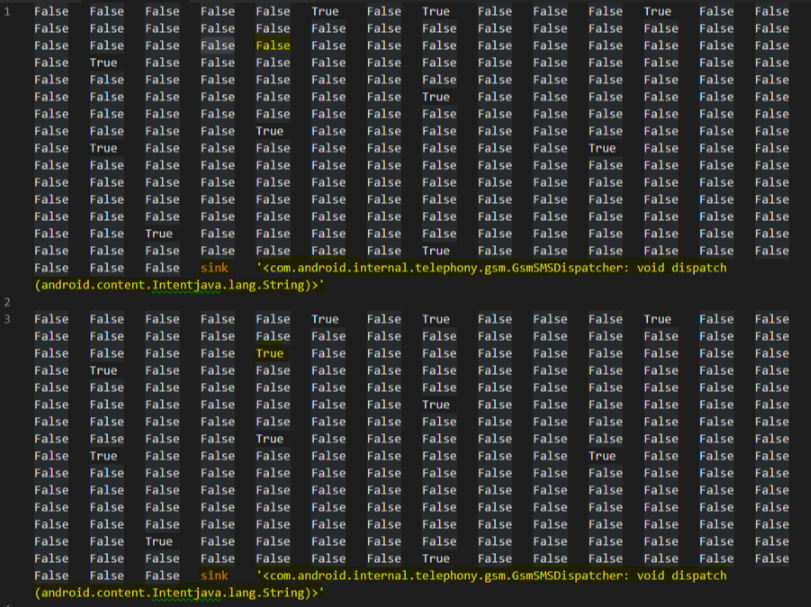
\includegraphics[width=0.9\linewidth]{images/menthod_though_apis.png}
    \caption{%
    Methods through different API Levels. We can observe in yellow the feature "Method modifier is PUBLIC" and the full method name. Even for different features values, marked in green, the method still belongs to the sink class.%
    }
\end{figure}\label{menthod_though_apis}

\section{Monolithic}\label{mono}

For the Monolithic classifiers, we have the Decision Tree, Multinomial and Bernoulli Naive Bayes, K-Nearest Neighbor (KNN), Support Vector Machine (SVM), Multi-Layer Perceptron and Random Forest.

The setup for Decision Tree is the split strategy to select the most relevant feature with Gini Impurity as criterion. In Multinomial and Bernoulli Naive Bayes we choose a $\alpha$ of 1. For KNN, we use 5 as the number of neighbors and a uniform weight for the neighbor points. The SVM has L2 as penalty, linear kernel, $C = 1$ and tolerance of $10^{-4}$. For MLP we used L2 regularization with alpha of $10^{-4}$, 1000 neurons in hidden layer, no early stopping, activation layer as relu, max of 1000 iterations and tolerance of $10^{-4}$. For Random Forests we are using 10 estimators, the minimum samples to split is 2 and Gini Impurity as criterion. The parameters can also be seen in Table \ref{table:monolithic_params}.

\begin{table}[h!]
    \centering
    \renewcommand{\arraystretch}{1.8}
    \begin{tabular}{ p{4cm}p{1.62cm}|p{1.5cm}|p{1.5cm}|p{1.5cm}|p{1.5cm} }
        \toprule
        Model & \multicolumn{5}{c}{Parameters} \\
        \midrule
        Decision Tree & criterion Gini & spliter best & & &\\
        Multinomial NB & $\alpha = 1$ & & & &\\
        Bernoulli NB & $\alpha = 1$ & & & &\\
        KNN & $ k = 5 $ & uniform weight & & &\\
        Linear SVM & penalty L2 & $C = 1$ & tolerance $10^{-4}$ & &\\
        MLP  & $ \alpha = 10^{-4} $ & reg. L2  & activation relu & tolerance $10^{-4}$ & hidden neurons 1000 \\
        Random Forest & criterion Gini & samples 2 & estimators 10 & & \\ [1ex]
        \bottomrule
        \end{tabular}
        \caption{%
        Parameters for Monolithic Classifiers%
        }\label{table:monolithic_params}
\end{table}

\begin{table}[h!]
    \centering
    \renewcommand{\arraystretch}{1.8}
    \begin{tabular}{ p{3cm}p{2.8cm}p{2.8cm}p{2.8cm}p{2.8cm} }
        \toprule
        Model & Precision & Recall & F1 Score & Accuracy \\
        \midrule
        Decision Tree & 0.8474 (0.0505) & 0.8388 (0.0549) & 0.8410 (0.0357) & 0.8497 (0.0217) \\
        Multinomial NB & 0.8297 (0.0595) & 0.8211 (0.0552) & 0.8231 (0.0416) & 0.8387 (0.0282) \\
        Bernoulli NB & 0.8307 (0.0609) & 0.8180 (0.0561) & 0.8220 (0.0424) & 0.8378 (0.0271) \\
        KNN & 0.8635 (0.0547) & 0.7991 (0.0657) & 0.8217 (0.0484) & 0.8432 (0.0307) \\
        Linear SVM & 0.8920 (0.0559) & 0.8718 (0.0539) & 0.8796 (0.0436) & 0.8859 (0.0284) \\
        MLP & 0.8936 (0.0547) & \textbf{0.8759 (0.0541)} & \textbf{0.8830 (0.0437)} & \textbf{0.8908 (0.0302)} \\
        Random Forest & \textbf{0.8953 (0.0568)} & 0.8522 (0.0605) & 0.8684 (0.0438) & 0.8791 (0.0309) \\ [1ex]
        \bottomrule
        \end{tabular}
        \caption{%
        Result for Monolithic Classifiers, Mean (Standard Deviation), the best classifier for each metric is highlighted in bold. Using the %
        }\label{table:result_monolithic}
\end{table}

The Table \ref{table:result_monolithic} is showing the results for Monolithic Classifiers. We can observe that the MLP has better results overall, just behind of Random Forest in precision by 0,0017. This interval is within the confidence interval, the standard deviation of MLP and Random Forest have the same approximation of 0.05. We can also observe that the SMV is close to MLP and Random Forest in all metrics, this is an evidence that SVM can solve this problem as well as these two.
\section{Multiple Classifier System}\label{mcs}

For the Multiple Classifier System we used KNORAE, KNORAU, META-DES, OLA, Single Best and Static Selection. Each of these algorithms has the objective to select the best classifier in a set, in our evaluation, we are using a pool of 100 classifiers of the same base class.

The base classifier classes used are Perceptron and Decision Tree, in all ensemble algorithms we use the same base classifier configuration. For Perceptron we used no regularization, no early stopping, max of 1000 iterations and tolerance of $10^{-1}$. For Decision Tree, the split strategy is to select the most relevant feature with Gini Impurity as criterion. For ensemble algorithms, the KNORAE and KNORAU parameters were KNN to estimate the classifier competence using 7 neighbors, with no dynamic pruning and no indecision region. For META-DES, we are using Multinomial Naive Bayes as meta-classifier, 5 output profiles to estimate the competence using a KNN with 7 neighbors to decide the region of competence. And finally, static selection, we are choosing 50\% of the base classifiers. All parameters can be seen in Table \ref{table:mcs_params}.

\begin{table}[h!]
    \centering
    \renewcommand{\arraystretch}{1.8}
    \begin{tabular}{ p{5cm}p{3cm}|p{3cm}|p{3cm} }
        \toprule
        Model & \multicolumn{3}{c}{Parameters} \\
        \midrule
        Perceptron & max iterations \newline 1000 & tolerance $10^{-4}$ & \\
        Decision Tree & criterion Gini & spliter best & \\
        \midrule
        KNORAE and KNORAU & $k = 7$ & no prune & no indecision \\
        META-DES & Multinom. NB & $K_p = 5$ & $k = 7$ \\
        Static Selection & selection 50\% & & \\
        \bottomrule
        \end{tabular}
        \caption{%
        Parameters for Multiple Classifier System%
        }\label{table:mcs_params}
\end{table}

In Table \ref{mcs_dt_table} is presented the MCS algorithms using Decision Tree classifier. We can observe a better mean result using META-DES in all metrics. Considering the mean and standard deviation, the results for KNORAE, OLA, Static Selection and META-DES are very close to the same interval.

When using Perceptron as main classifier, Table \ref{mcs_perceptron_table}, we can observe that KNORAE and META-DES have the best mean results, META-DES has better Precision ad Accuracy and KNORAE has better Recall and F1 Score. But also, when considering the mean and standard deviation, the results are in the same range comparing KNORAE, KNORAU, OLA and Static Selection.Comparing both Decision Tree and Perceptron results in MCS, the results are very close, having 0.8665(0.0316) as F1 Score for the best Perceptron MCS (KNORAE) and 0.8741(0.0284) for the best Decision Tree MCS (META-DES), a difference of just 0.0086.

\begin{table}[h!]
    \centering
    \renewcommand{\arraystretch}{1.8}
    \begin{tabular}{ p{3cm}p{2.8cm}p{2.8cm}p{2.8cm}p{2.8cm} }
        \toprule
        Model & Precision & Recall & F1 Score & Accuracy \\
        \midrule
        KNORAE &            0.8602 (0.0517) & 0.8395 (0.0656) & 0.8469 (0.0455) & \textbf{0.8580 (0.0306)} \\
        KNORAU &            0.8377 (0.0557) & 0.8071 (0.0743) & 0.8181 (0.0495) & 0.8313 (0.0321) \\
        META-DES &          \textbf{0.8609 (0.0551)} & \textbf{0.8423 (0.0639)} & \textbf{0.8492 (0.0482)} & 0.8575 (0.0344) \\
        OLA &               0.8263 (0.0589) & 0.8104 (0.0667) & 0.8158 (0.0532) & 0.8306 (0.0387) \\
        Single Best &       0.7609 (0.0739) & 0.7356 (0.0994) & 0.7423 (0.0688) & 0.7629 (0.0447) \\
        Static Selection &  0.8424 (0.0579) & 0.8099 (0.0741) & 0.8213 (0.0492) & 0.8338 (0.0341) \\ [1ex]
        \bottomrule
        \end{tabular}
        \caption{%
        Result for Multiple Classifier System, Mean (Standard Deviation), using Decision Tree as main classifier with most relevant feature as split strategy and Gini Impurity as criterion. The best classifier for each metric is highlighted in bold%
        }\label{mcs_dt_table}
\end{table}

\begin{table}[h!]
    \centering
    \renewcommand{\arraystretch}{1.8}
    \begin{tabular}{ p{3cm}p{2.8cm}p{2.8cm}p{2.8cm}p{2.8cm} }
        \toprule
        Model & Precision & Recall & F1 Score & Accuracy \\
        \midrule
        KNORAE &            0.8607 (0.0556) & \textbf{0.8368 (0.0678)} & \textbf{0.8452 (0.0471)} & \textbf{0.8570 (0.0273)} \\
        KNORAU &            0.8446 (0.0562) & 0.8148 (0.0581) & 0.8260 (0.0451) & 0.8386 (0.0301) \\
        META-DES &          \textbf{0.8748 (0.0559)} & 0.8167 (0.0700) & 0.8375 (0.0518) & 0.8525 (0.0335) \\
        OLA &               0.8418 (0.0580) & 0.8216 (0.0550) & 0.8282 (0.0413) & 0.8410 (0.0268) \\
        Single Best &       0.7913 (0.0753) & 0.7552 (0.1007) & 0.7644 (0.0688) & 0.7866 (0.0451) \\
        Static Selection &  0.8523 (0.0593) & 0.8158 (0.0717) & 0.8291 (0.0512) & 0.8438 (0.0329) \\ [1ex]
        \bottomrule
        \end{tabular}
        \caption{%
        Result for Multiple Classifier System, Mean (Standard Deviation), using Perceptron as main classifier using no regularization, no early stopping, max of 1000 iterations and tolerance of $10^{-1}$. The best classifier for each metric is highlighted in bold%
        }\label{mcs_perceptron_table}
\end{table}
\section{Final Considerations}\label{result_ending}

With the Monolithic and MCS compared, now we must compare the best Monolithic and the best MCS to fully understand which model is the most indicated to solve the problem of Android API methods categorization. Table \ref{table:overall_comp} show the performance of each classifier: MLP and METADES using Decision Tree, and we can see that the MLP has better results in all the metrics.

\begin{table}[hb]
    \centering
    \renewcommand{\arraystretch}{1.8}
    \begin{tabular}{ p{3cm}p{2.8cm}p{2.8cm}p{2.8cm}p{2.8cm} }
        \toprule
        Model & Precision & Recall & Accuracy & F1 Score \\
        \midrule
        MLP &       \textbf{0.8838 (0.0474)} & \textbf{0.8709 (0.0544)} & \textbf{0.8758 (0.0426)} & \textbf{0.8856 (0.0287)} \\
        META-DES \newline Decision Tree &  0.8609 (0.0551) & 0.8423 (0.0639) & 0.8492 (0.0482) & 0.8575 (0.0344) \\
        \bottomrule
    \end{tabular}
    \caption{%
        The best of Monolithic compared to the best of MCS, Mean (Standard Deviation). The best classifier for each metric is highlighted in bold.
        %
    }\label{table:overall_comp}
\end{table}

\begin{table}[!ht]
    \centering
    \renewcommand{\arraystretch}{1.8}
    \begin{tabular}{ p{2.2cm}p{0.8cm}p{2.7cm}p{2.7cm}p{2.7cm}p{2.7cm} }
        \toprule
        Model & Class & Precision & Recall & Accuracy & F1 Score \\
        \midrule
        \multirow{3}{*}{MLP}
        & (1) & 0.8792 (0.0597) & \textbf{0.8708 (0.0786)} & \textbf{0.8731 (0.0577)} & \textbf{0.8856 (0.0287)} \\
        & (2) & \textbf{0.8803 (0.0486)} & \textbf{0.8219 (0.0598)} & \textbf{0.8489 (0.0450)} & \textbf{0.8856 (0.0287)} \\
        & (3) & \textbf{0.8920 (0.0339)} & \textbf{0.9200 (0.0248)} & \textbf{0.9055 (0.0251)} & \textbf{0.8856 (0.0287)} \\
        \midrule
        \multirow{3}{*}{\shortstack{METADES\\Decision Tree }}
        & (1) & \textbf{0.8870 (0.0658)} & 0.8611 (0.0889) & 0.8702 (0.0580) & 0.8575 (0.0344) \\
        & (2) & 0.8344 (0.0636) & 0.7676 (0.0691) & 0.7983 (0.0579) & 0.8575 (0.0344) \\
        & (3) & 0.8614 (0.0361) & 0.8982 (0.0338) & 0.8790 (0.0288) & 0.8575 (0.0344) \\
        \bottomrule
        \end{tabular}
        \caption{%
        C The best of Monolithic compared to the best of MCS, Mean (Standard Deviation). The Class (1) represents the Source methods, Class (2) are the Sink methods and (3) Neithernor. The best classifier for each metric and class is highlighted in bold.
        %
        }\label{table:per_class_overall_comp}
\end{table}

Looking deep to the results for each class, we can observe in Table \ref{table:per_class_overall_comp} that the MLP has a better score in the majority of classes and metrics and METADES using Decision Tree as base classifier has better Precision when classifying the Source methods. If we look at the standard deviation, we can conclude that the classifiers are also in the same interval for all the metrics, this is another evidence that a simpler algorithm can address this problem.
